\documentclass[addpoints]{exam}
\usepackage[a4paper]{geometry}
\usepackage{amsmath}
\usepackage{amssymb}
\usepackage{amsthm}
\usepackage{calc}
\usepackage{enumitem}
\usepackage{tikz}
\usepackage{float}
\usepackage{titling}
\usepackage{listings}
\usepackage{pdfpages}
\usepackage{setspace}
\usepackage{comment}
\usepackage{pgfplots}
\pgfplotsset{width=10cm,compat=1.9}
\usepackage{xcolor}
\usepackage{ amssymb }
\usepackage{tikz}
\usepackage{lmodern}
\pagestyle{headandfoot}
\runningheadrule
\runningfootrule
\runningheader{PHY 202}{}{\theauthor}
\runningfooter{}{\thepage}{}
\firstpageheader{}{}{}

\boxedpoints
\printanswers

\newcommand\mbb[1]{\ensuremath{\mathbb{#1}}}
\usepgfplotslibrary{external}
\tikzexternalize 
\title{Quantum Mechanics Assignment 3}
\author{Muhammad Meesum Ali Qazalbash - mq06861}
\date{}
\renewcommand{\qedsymbol}{\ensuremath{\blacksquare}}

\begin{document}
\maketitle
\begin{questions}
    \question[15] Consider the wave function:
    \[\Psi(x,t)=Ae^{-\lambda|x|}e^{-i\omega t}\]
    where $A$, $\lambda$ and $\omega$ are positive real numbers.
    \begin{enumerate}
        \item Normalize $\Psi$.
        \item Determine the expression values of $x$ and $x^2$.
        \item Find the standard deviation of $x$. Sketch the graph of $\Psi$ as a function of $x$, and mark the points $\langle\langle x\rangle+\sigma\rangle$ and $\langle\langle x\rangle-\sigma\rangle$ to to illustrate the sense in which $\sigma$ represent the \"spread\" of $x$. What is the probability that the particle would be found outside this range?
    \end{enumerate}
    \begin{solution}
        We would first find the coefficient $A$ for normalization,
        \begin{align*}
                     & \int_{-\infty}^{\infty} {|\Psi(x,t)|}^2 dx                                                                            = 1              \\
            \iff     & \int_{-\infty}^{\infty} {\Psi(x,t)}{{\Psi}^{*}(x,t)} dx                                                               = 1              \\
            \iff     & \int_{-\infty}^{\infty} {\left(Ae^{-\lambda|x|}e^{-i\omega t}\right)}{\left(Ae^{-\lambda|x|}e^{i\omega t}\right)} dx  = 1              \\
            \iff     & \int_{-\infty}^{\infty} {\left(Ae^{-\lambda|x|}\right)}{\left(Ae^{-\lambda|x|}\right)} dx                             = 1              \\
            \iff     & A^2 \int_{-\infty}^{\infty} {e^{-2\lambda|x|}} dx                                                                     = 1              \\
            \iff     & A^2 \int_{-\infty}^{0} {e^{2\lambda x}} dx + A^2 \int_{0}^{\infty} {e^{-2\lambda x}} dx                               = 1              \\
            \iff     & \frac{A^2}{2\lambda}e^{2\lambda x}\Big|_{-\infty}^{0} - \frac{A^2}{2\lambda}e^{-2\lambda x}\Big|_{0}^{\infty}         = 1              \\
            \implies & \frac{A^2}{\lambda}                                                                                                   = 1              \\
            \implies & A                                                                                                                     = \sqrt{\lambda}
        \end{align*}
        Therefore the normalized wavefunction is,
        \begin{align*}
            \Psi(x,t) & = \sqrt{\lambda}e^{-\lambda |x|-i\omega t}
        \end{align*}
        The probability density function for a given wave function is defined as,
        \[P[X=x] = |\Psi(x,t)|^2\]
        From the analysis in the previous part,
        \[P[X=x] = \lambda e^{-2\lambda|x|}\]
        The expectation of $x$ is therefore given by,
        \begin{align*}
            \langle x \rangle & = \int_{-\infty}^{\infty} xP[X=x] dx                                                            \\
                              & = \int_{-\infty}^{\infty} x\lambda e^{-2\lambda|x|} dx                                          \\
                              & = \int_{-\infty}^{0} x\lambda e^{2\lambda x} dx + \int_{0}^{\infty} x\lambda e^{-2\lambda x} dx \\
                              & = -\frac{1}{4\lambda} + \frac{1}{4\lambda}                                                      \\
                              & = 0
        \end{align*}
        And the expectation of $x^2$ is given by;
        \begin{align*}
            \langle x^2 \rangle & = \int_{-\infty}^{\infty} x^2P[X=x] dx                                                              \\
                                & = \int_{-\infty}^{\infty} x^2\lambda e^{-2\lambda|x|} dx                                            \\
                                & = \int_{-\infty}^{0} x^2\lambda e^{2\lambda x} dx + \int_{0}^{\infty} x^2\lambda e^{-2\lambda x} dx \\
                                & = \frac{1}{4\lambda ^2} + \frac{1}{4\lambda ^2}                                                     \\
                                & = \frac{1}{2\lambda ^2}
        \end{align*}
        The plot for the probability density function is as follows:


        \begin{figure}[H]
            %       \centering
            %       \begin{tikzpicture}
            %           \begin{axis}[
            %                   xmin = -2, xmax = 2,
            %                   ymin = 0, ymax = 1.0]
            %               \addplot[
            %                   domain = -2:2,
            %                   samples = 200,
            %                   smooth,
            %                   thick,
            %                   blue,
            %               ] {exp(-2 * abs(x))};
            %           \end{axis}
            %       \end{tikzpicture}

            %       \caption{Probability Distribution function}
            %       \label{Probability Distribution function q1}

            \centering
            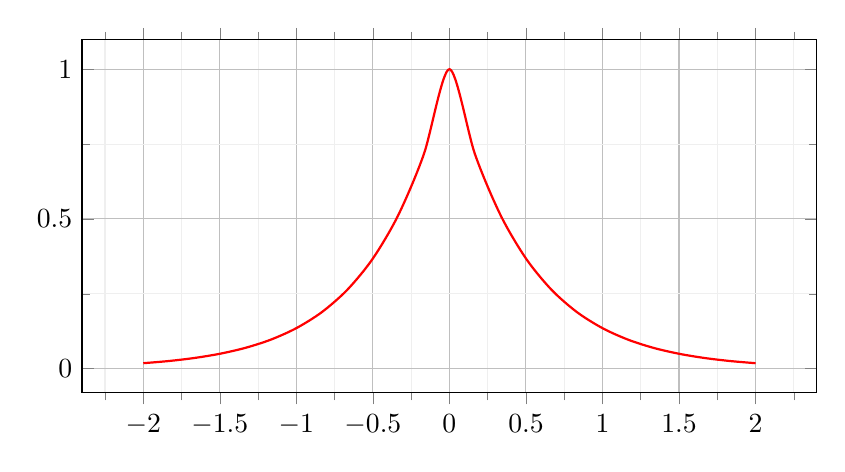
\begin{tikzpicture}
                \begin{axis} [
                        ybar,
                        grid = both,
                        minor tick num = 1,
                        major grid style = {lightgray},
                        minor grid style = {lightgray!25},
                        width = 0.9\textwidth,
                        height = 0.5\textwidth
                    ]
                    \addplot [
                        domain = -2:2,
                        smooth,
                        thick,
                        red,
                    ]  {exp(-2 * abs(x))};
                \end{axis}
            \end{tikzpicture}
            \caption{Probability Distribution function}
        \end{figure}

        The standard deviation for $P[X=x]$ is given as,
        \begin{align*}
            \sigma & = \sqrt{\langle x^2 \rangle - {\langle x \rangle}^2} \\
                   & = \sqrt{\frac{1}{2\lambda ^2} - 0}                   \\
                   & = \frac{1}{\sqrt{2}\lambda}
        \end{align*}
        \noindent  According to the plot attached above, the probability that the particle would be found outside this range can be calculated as;
        \begin{align*}
            P[|X - \langle x \rangle| > \sigma] & =  \left(\int_{-\infty}^{\langle x \rangle - \sigma} + \int_{\langle x \rangle + \sigma}^{\infty}\right) {|\Psi(x,t)|^2} dx                        \\
                                                & = \lambda \int_{-\infty}^{-\frac{1}{\sqrt{2}\lambda}} {e^{2\lambda x}} dx + \lambda \int_{\frac{1}{\sqrt{2}\lambda}}^{\infty} {e^{-2\lambda x}} dx \\
                                                & = \frac{e^{-\sqrt{2}}}{2} + \frac{e^{-\sqrt{2}}}{2}                                                                                                \\
                                                & = e^{-\sqrt{2}} \approx 0.243
        \end{align*}

    \end{solution}
    \pagebreak
    \question[15] At the time $t = 0$, the particle waver function is represented by :
    \[\Psi(x,0)=\begin{cases}
            Ax/a         & \text{if } 0 \leq x \leq a \\
            A(b-x)/(b-a) & \text{if } a \leq x \leq b \\
            0            & \text{otherwise}
        \end{cases}\]
    where $A$, $a$, and $b$ are constants.
    \begin{enumerate}
        \item Normalise $\Psi$, that is $A$ in terms of $a$ and $b$.
        \item Sketch $\Psi(x, 0)$ as a function of $x$.
        \item Where is the particle most likely to be found at $t = 0$ ?
        \item what is the probability of finding the particle to the left of $a$ ? Check your results in the limiting cases when $b = a$ and $b = 2a$.
        \item What is the expectation value of $x$ ?
    \end{enumerate}

    \begin{solution}

        We would first find the coefficient $A$ for normalization,
        \begin{align*}
                 & \int_{-\infty}^{\infty} {|\Psi(x,t)|}^2 dx                                                          = 1                                                     \\
            \iff & \left(\int_{-\infty}^{0}+\int_{0}^{a}+\int_{a}^{b}+\int_{b}^{\infty}\right) {|\Psi(x,t)|}^2 dx                                                          = 1 \\
            \iff & \int_{0}^{a} {|\Psi(x,t)|}^2 dx + \int_{a}^{b} {|\Psi(x,t)|}^2 dx                                   = 1                                                     \\
            \iff & \int_{0}^{a} {\Bigg|A\frac{x}{a}\Bigg|}^2 dx + \int_{a}^{b} {\Bigg|A\frac{b-x}{b-a}\Bigg|}^2 dx = 1                                                         \\
            \iff & \frac{A^2}{a^2} \int_{0}^{a} x^2 dx + \frac{A^2}{(b-a)^2} \int_{a}^{b} (b-x)^2                      = 1                                                     \\
            \iff & A^2\left(\frac{a^3}{3a^2} + \frac{(b-a)^3}{3(b-a)^2}\right)                                         = 1                                                     \\
            \iff & A^2\left(\frac{a + b - a}{3}\right)                                                                 = 1                                                     \\
            \iff & A                                                                                                   = \sqrt{\frac{3}{b}}
        \end{align*}
        The Schrodinger equation at t = 0 is given by;
        \begin{figure}[H]
            %       \centering
            %       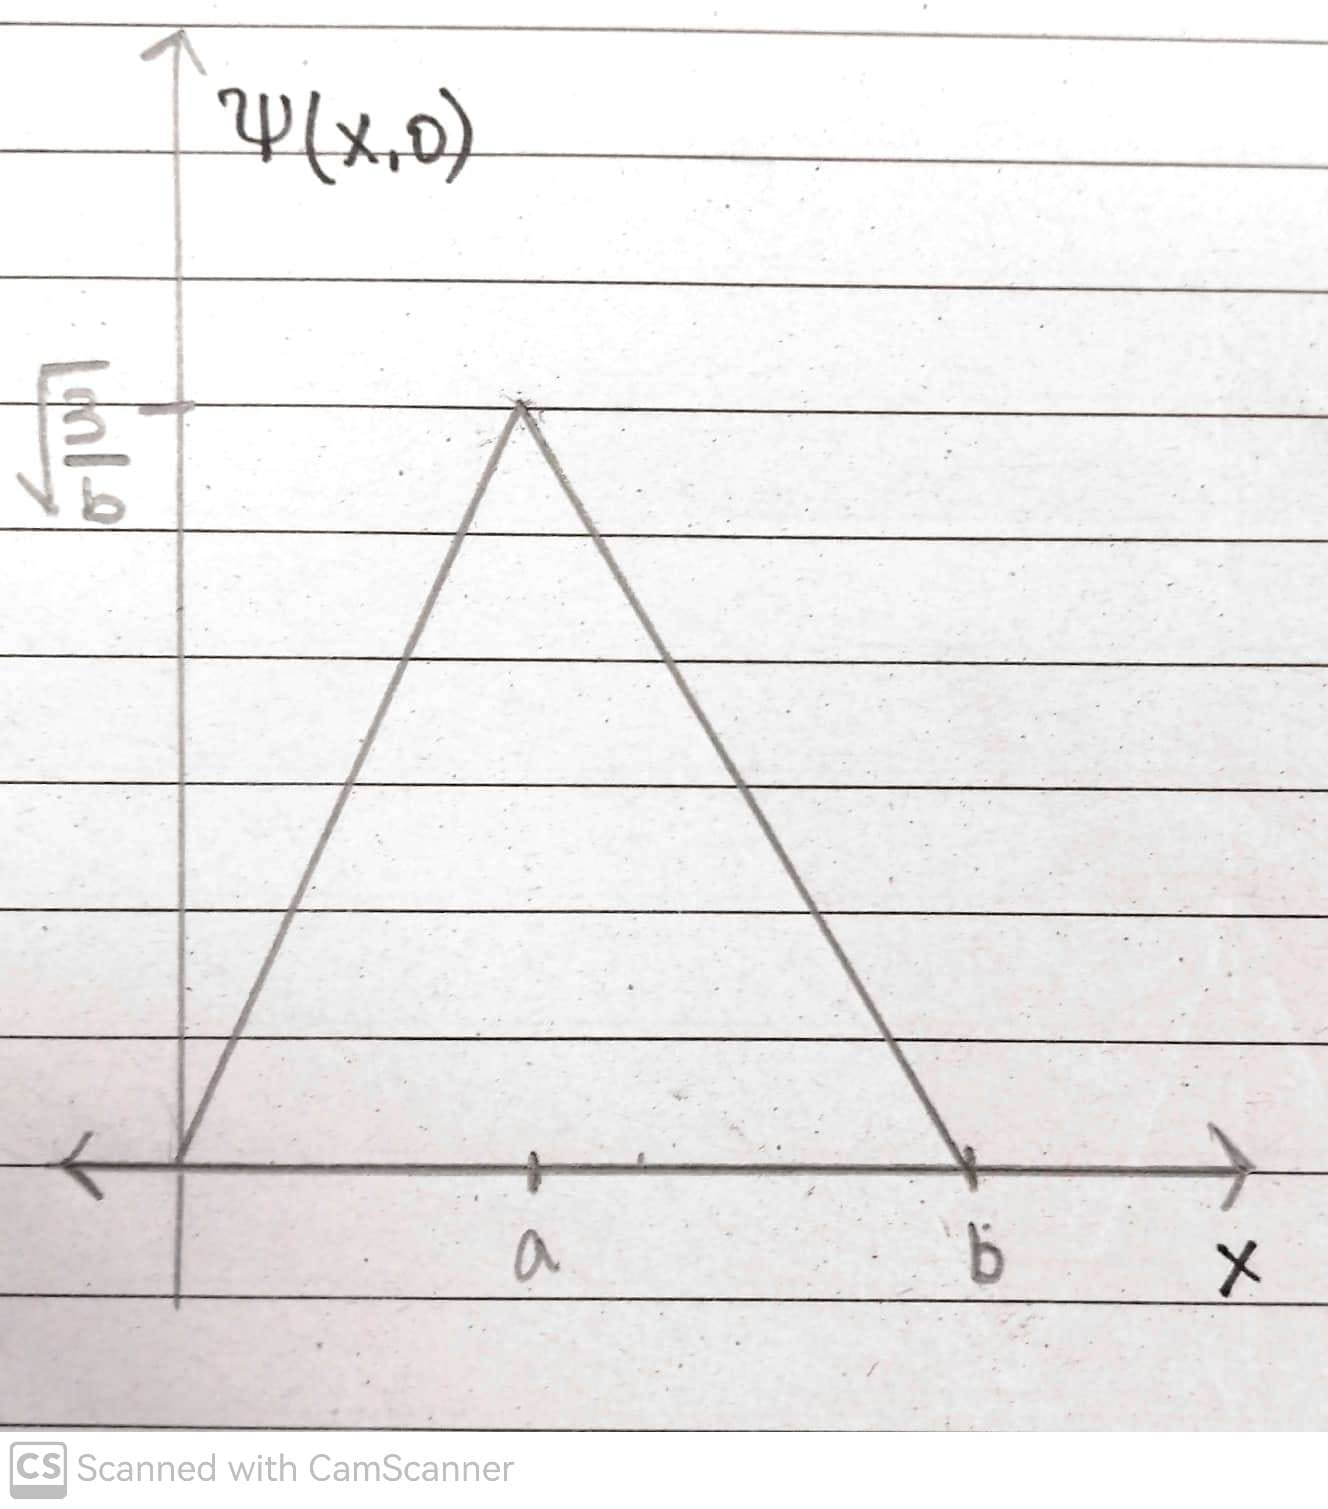
\includegraphics[scale = 0.1]{assignment 3 q2 schrodinger.jpeg}
            %       \caption{Probability Distribution function}
            %       \label{Probability Distribution function q21}
            \centering
            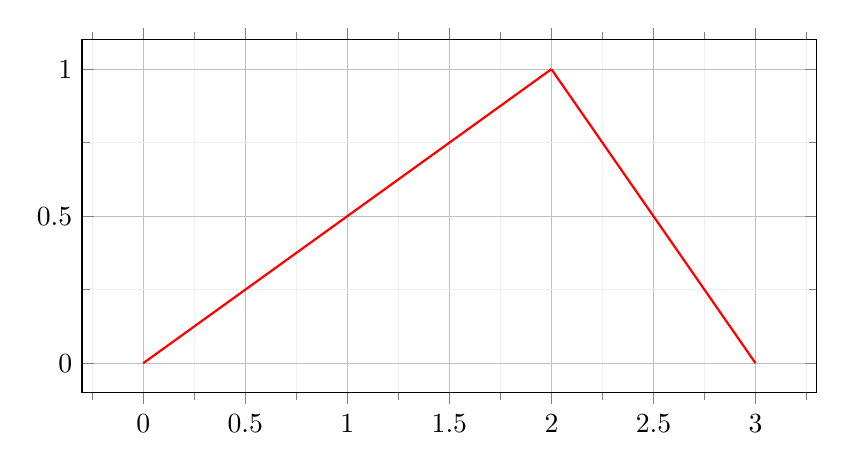
\begin{tikzpicture}
                \begin{axis} [
                        ybar,
                        grid = both,
                        minor tick num = 1,
                        major grid style = {lightgray},
                        minor grid style = {lightgray!25},
                        width = 0.9\textwidth,
                        height = 0.5\textwidth
                    ]
                    \addplot [
                        domain = 0:2,
                        smooth,
                        thick,
                        red,
                    ]  {x/2};
                    \addplot [
                        domain = 2:3,
                        smooth,
                        thick,
                        red,
                    ]  {3-x};
                \end{axis}
            \end{tikzpicture}
            \caption{Probability Distribution function}
        \end{figure}
        The plot for the probability density function is as follows:
        \begin{figure}[H]
            %       \centering
            %       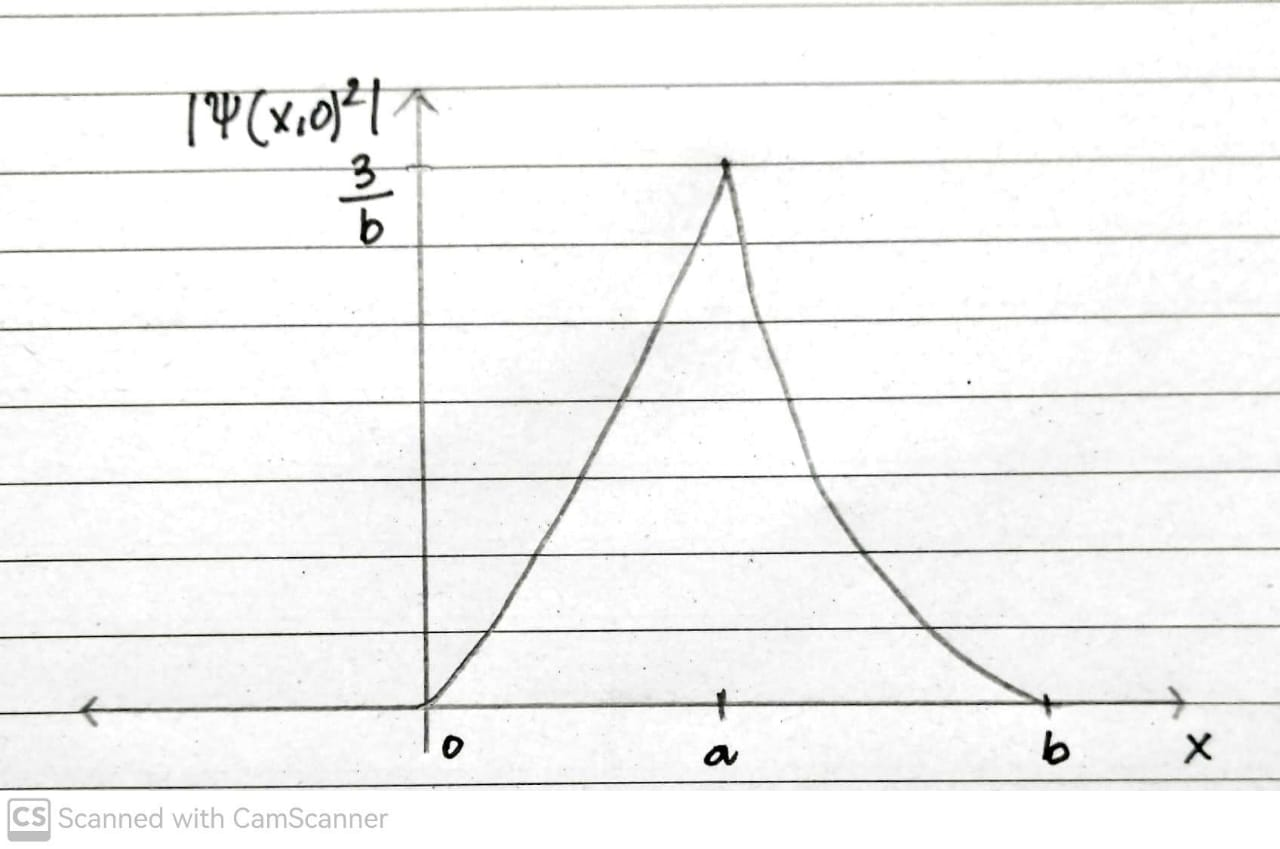
\includegraphics[scale = 0.25]{assignment 3 q2.jpeg}
            %       \caption{Probability Distribution function}
            %       \label{Probability Distribution function q22}
            % \begin{center}
            \centering
            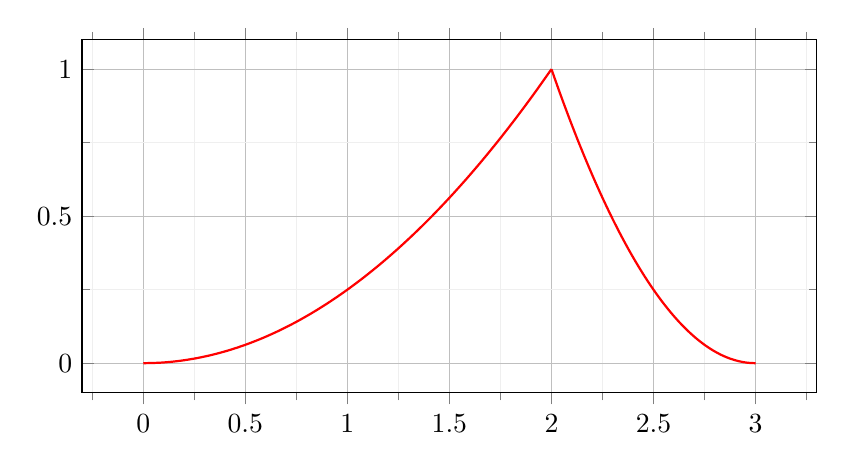
\begin{tikzpicture}
                \begin{axis} [
                        ybar,
                        grid = both,
                        minor tick num = 1,
                        major grid style = {lightgray},
                        minor grid style = {lightgray!25},
                        width = 0.9\textwidth,
                        height = 0.5\textwidth
                    ]
                    \addplot [
                        domain = 0:2,
                        smooth,
                        thick,
                        red,
                    ]  {x^2/4};
                    \addplot [
                        domain = 2:3,
                        smooth,
                        thick,
                        red,
                    ]  {(3-x)^2};
                \end{axis}
            \end{tikzpicture}
            \caption{Probability Distribution function}
        \end{figure}
        It can be seen in the graph attached above that at $t = 0$, the particle is most likely to be found at $x = a$.
        The probability of finding the particle to the left of $a$ can be given as;
        \begin{align*}
            P[X<a] & = \int_{-\infty}^{a} {|\Psi(x,t)|}^2 dx                          \\
                   & = \int_{0}^{a} {\left(\sqrt{\frac{3}{b}}\frac{x}{a}\right)}^2 dx \\
                   & = \frac{a}{b}
        \end{align*}
        When $b = a$, $P[X<a] = 1$ and when $b = 2a$, $P[X<a] = 0.5$.
        The expectation of $x$ can be found as;
        \begin{align*}
            \langle x \rangle & = \int_{-\infty}^{\infty} xP[X=x] dx                                                                                                \\
                              & = \int_{0}^{a} x\left(\sqrt{\frac{3}{b}}\frac{x}{a}\right)^2 dx + \int_{a}^{b} x\left(\sqrt{\frac{3}{b}}\frac{b-x}{b-a}\right)^2 dx \\
                              & = \frac{3}{a^2b}\frac{a^4}{4} - \frac{3}{b(b-a)^2}\left(\frac{b^4}{12} -\frac{6a^2b^2 - 8a^3b + 3a^4}{12}\right)                    \\
                              & = \frac{3a^2}{4b} +  \frac{3}{b(b-a)^2}\frac{(b-a)^3(b+3a)}{12}                                                                     \\
                              & = \frac{3a^2}{4b} + \frac{3(b-a)(b+3a)}{12b}                                                                                        \\
                              & = \frac{9a^2 + 3b^2 + 6ab - 9a^2}{12b}                                                                                              \\
                              & = \frac{6a+3b}{12}                                                                                                                  \\
                              & = \frac{2a+b}{4}
        \end{align*}

    \end{solution}
\end{questions}
% 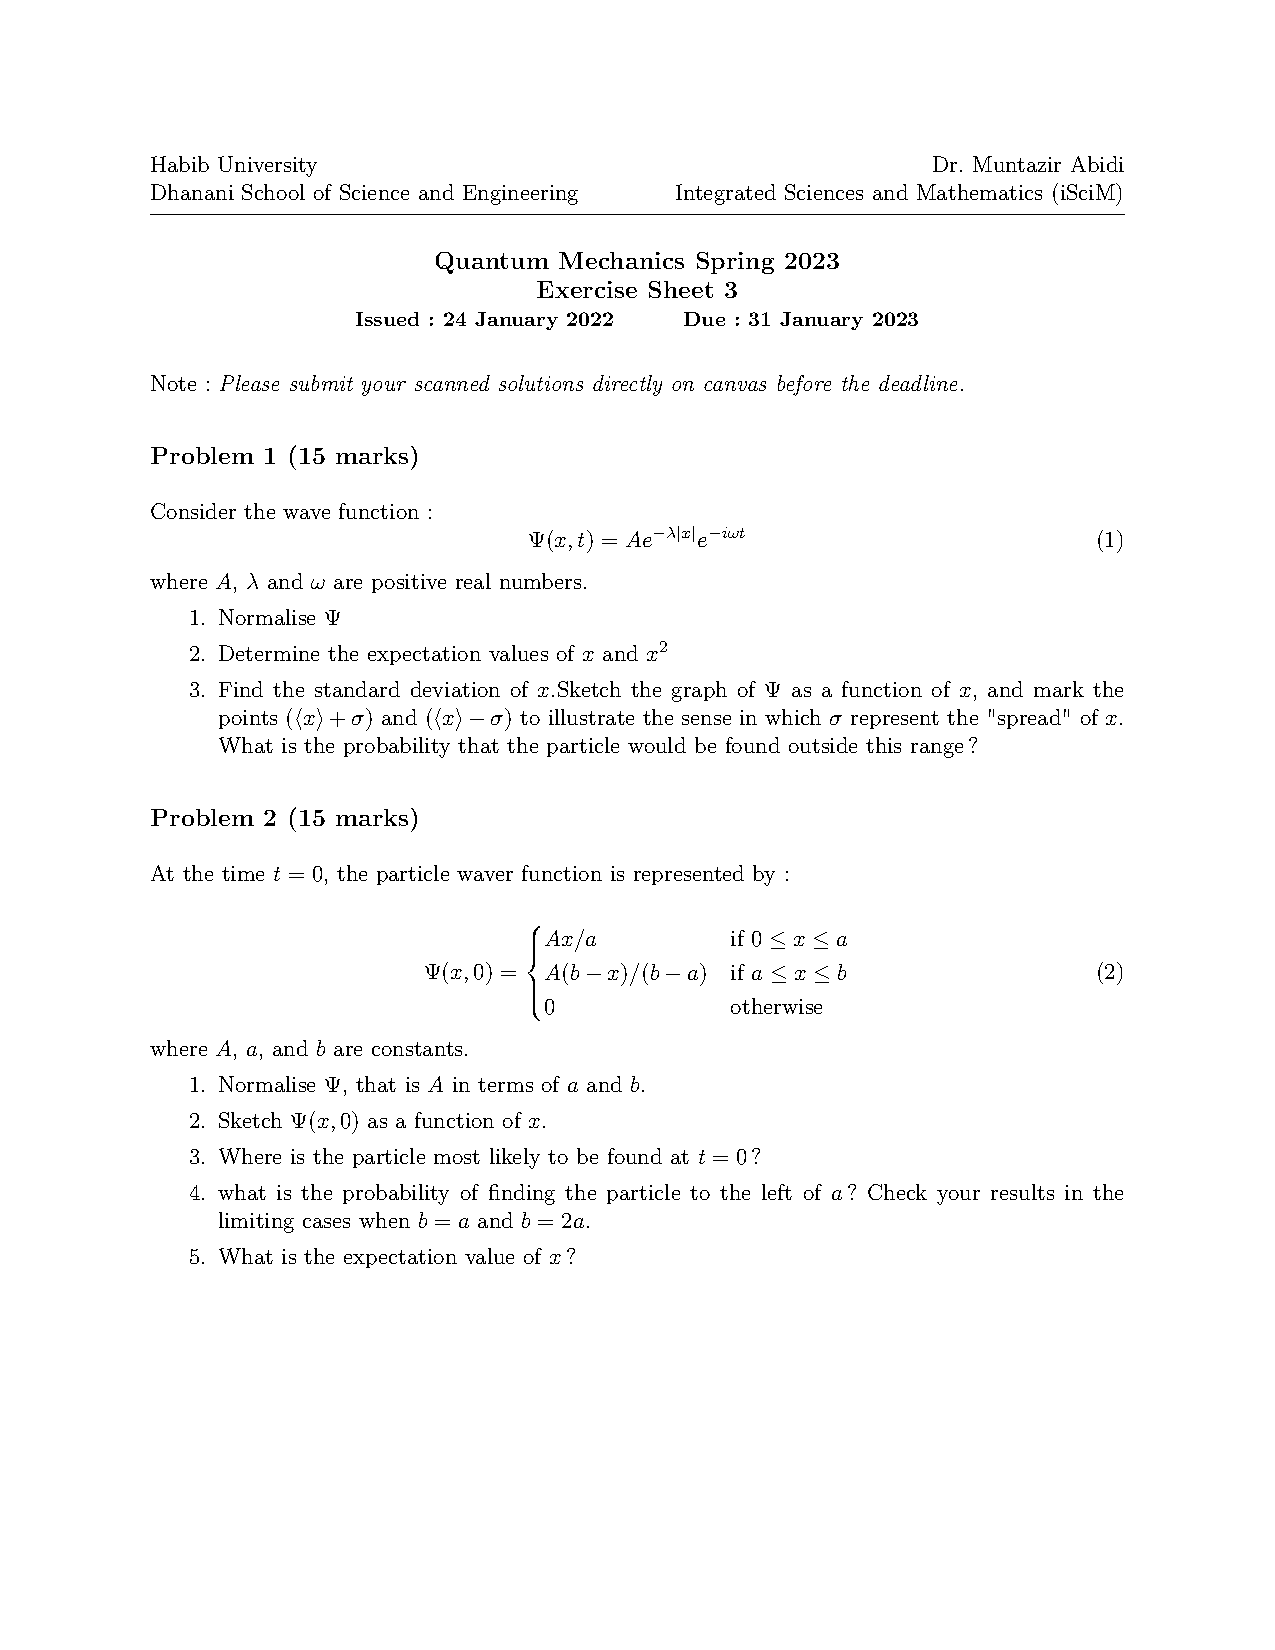
\includepdf[pages=-]{Assignment3_QM.pdf}
\end{document}
